%!TEX root = supplement.tex

%%%%%%%%%%%%%%%%%%%
\begin{figure}
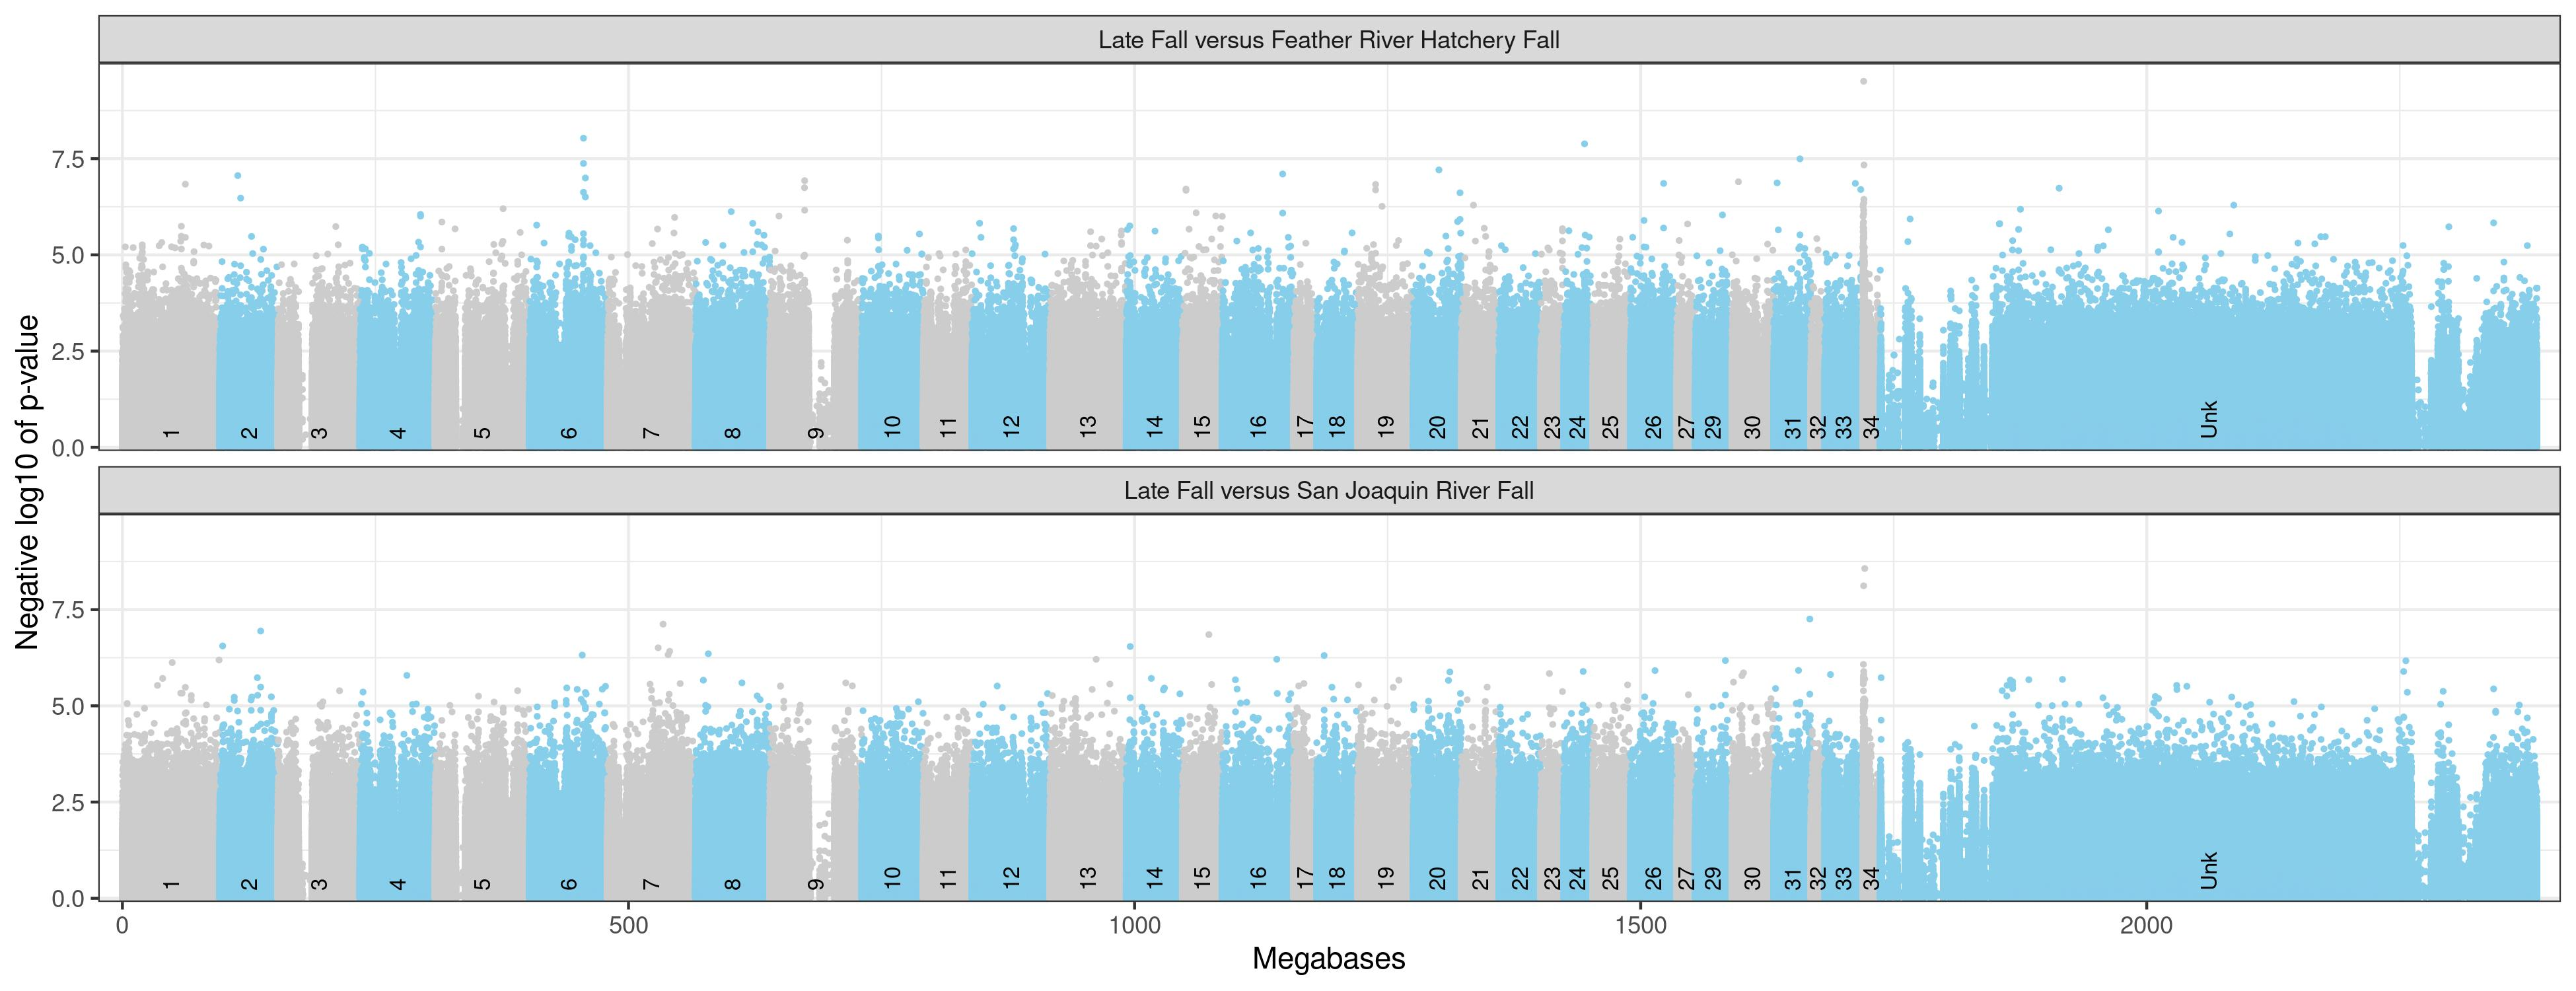
\includegraphics[width=\textwidth]{images/lfar-assoc-faceted.jpg}
\caption[
	Negative log base 10 of association $p$-values for
	individual SNPs for late-fall versus fall run
]{
	\footnotesize Negative log base 10 of association $p$-values for
	individual SNPs for late-fall versus fall run.  $x$ axis shows position in genome (in megabases),
	with color alternating by chromosome, as indicated by numbers above the $x$-axis. ``Unk'' refers
	to unplaced scaffolds in the Otsh\_v1.0 genome assembly \citep{christensen2018chinook}. The 
	upper panel is the comparison between late-fall and Feather River Hatchery fall, while the lower 
	panel is the comparison of late-fall to San Joaquin River fall. 
}
\label{fig:lfar-assoc}
\end{figure}



%%%%%%%%%%%%%%%%%%%%%% 
\begin{figure}
\begin{center}
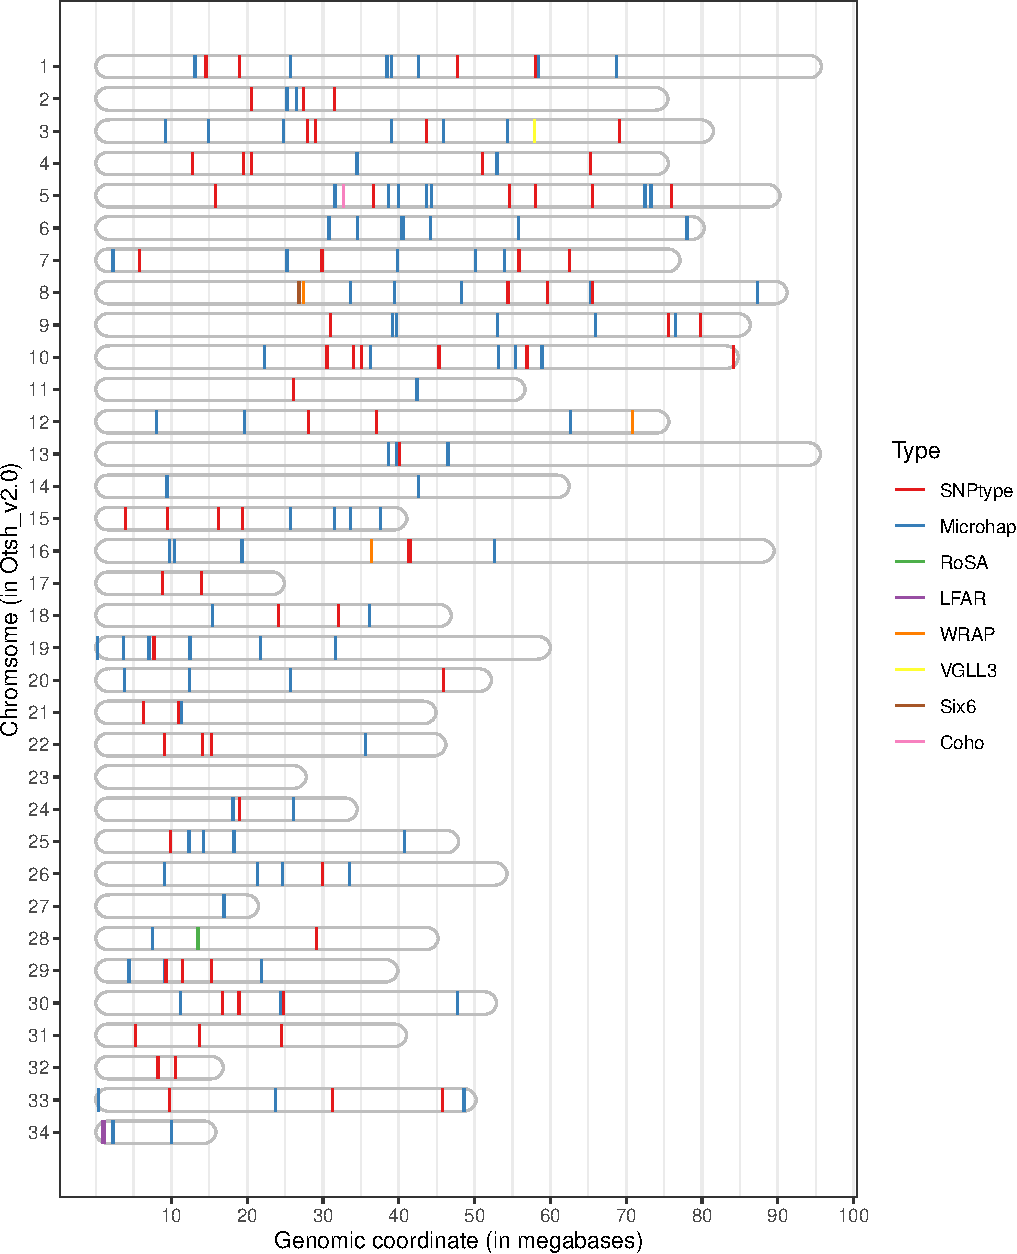
\includegraphics[width=0.7\textwidth]{images/genomic-locations-plot.pdf}
\end{center}
\caption[Genomic locations of amplicons]{\footnotesize Genomic locations of amplicons in the
Otsh\_v2.0 assembly of the Chinook salmon genome.  Color shows type of marker (see main text).
The sex-ID marker is not included here because it aligns to a scaffold that is not part of a
named chromosome/linkage group in the assembly.}
\label{fig:num-alle}
\end{figure}
%%%%%%%%%%%%%%%%%%%%





%%%%%%%%%%%%%%%%%%%%%% 
\begin{figure}
\begin{center}
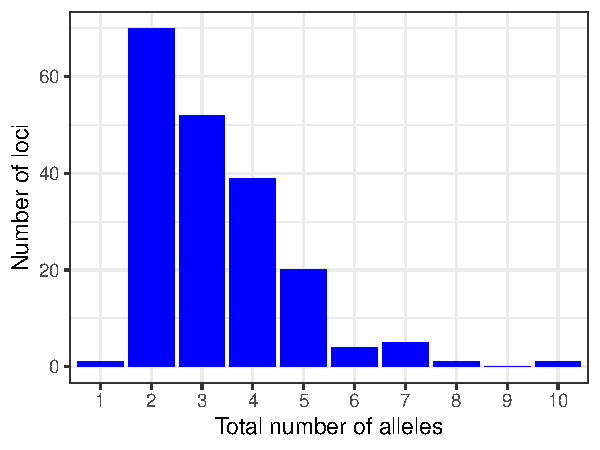
\includegraphics[width=0.7\textwidth]{images/num-alle-barplot.pdf}
\end{center}
\caption[Number of loci with different
total numbers of alleles]{\footnotesize Number of loci with different
total numbers of alleles in the data set. The one amplicon with only
one allele is {\tt Ots\_coho001\_05\_32691399}, which is fixed for alternate alleles
in Chinook vs.\ coho salmon. It is helpful in identifying coho samples that are
misidentified during sampling as Chinook salmon.}
\label{fig:num-alle}
\end{figure}
%%%%%%%%%%%%%%%%%%%%




%%%%%%%%%%%%%%%%%%%%%% 
\begin{figure}
\begin{center}
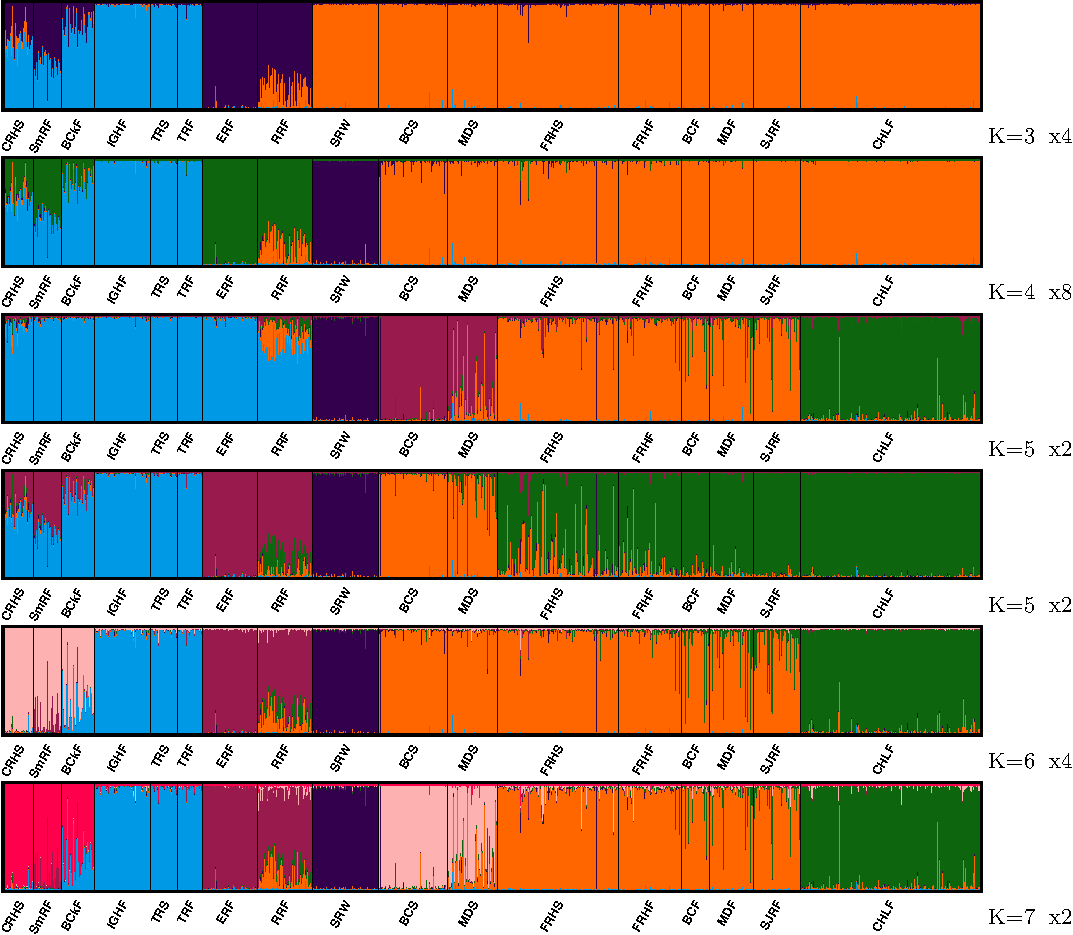
\includegraphics[width=0.7\textwidth]{images/minor-modes-crop.pdf}
\end{center}
\caption[STRUCTURE minor modes found by CLUMPAK]{\footnotesize STRUCTURE minor modes found by CLUMPAK.
At each value of $K$ for which a minor mode was found, the plot is shown.  $K$ values and number of times each minor
mode appeared out of 20 replicate runs of STRUCTURE appear to the lower right of each.}
\label{fig:minor-modes}
\end{figure}
%%%%%%%%%%%%%%%%%%%%


%%%%%%%%%%%%%%%%%%%%%% 
\begin{figure}
\begin{center}
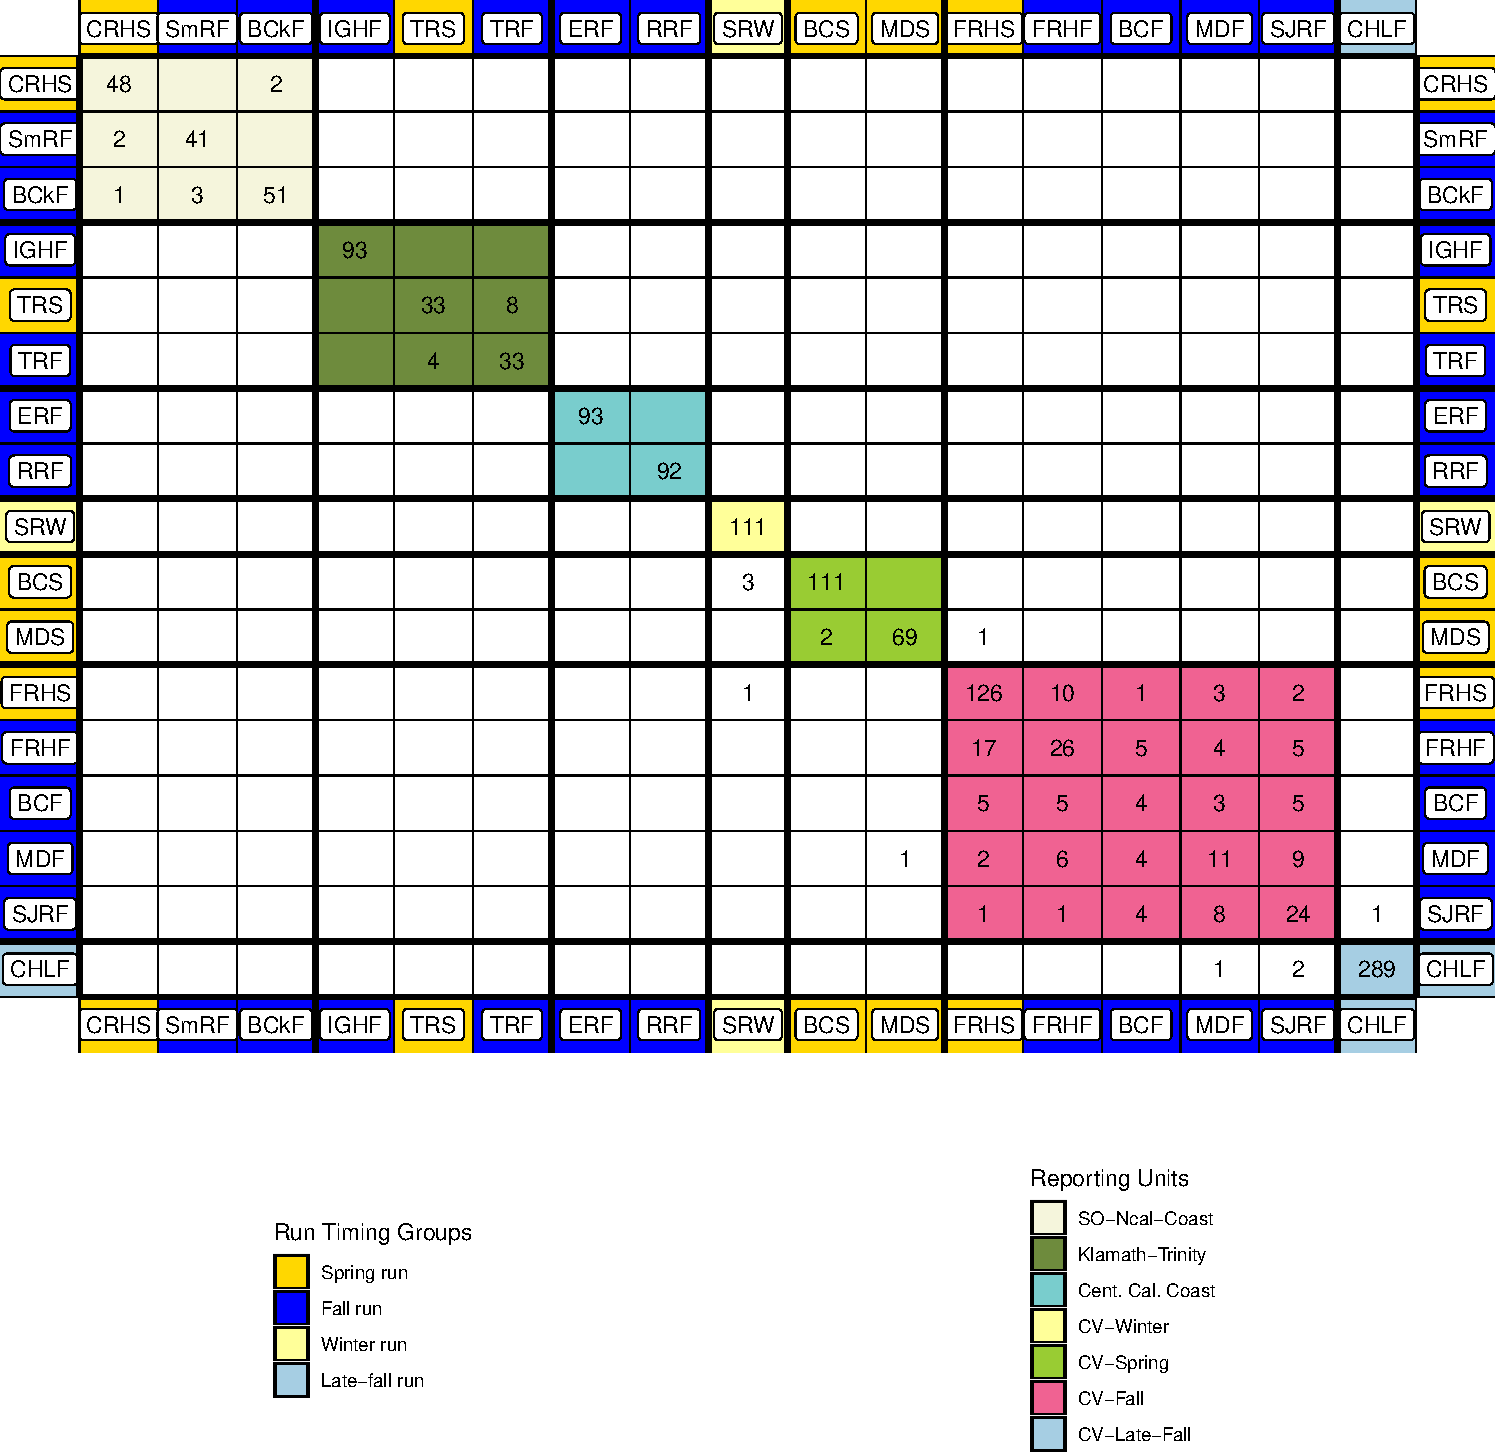
\includegraphics[width=0.8\textwidth]{images/ass-table-80-crop.pdf}
\end{center}
\caption[Assignment table for fish with scaled likelihood $ > 0.8$]{\footnotesize Assignment table
like that in Figure~\ref{fig:gsi}b in the paper, but constrained so that only fish assigning
to a reporting unit with scaled likelihood greater than 0.8 are included.}
\label{fig:eighty}
\end{figure}
%%%%%%%%%%%%%%%%%%%%





%%%%%%%%%%%%%%%%%%%%%% 
\begin{figure}
\begin{center}
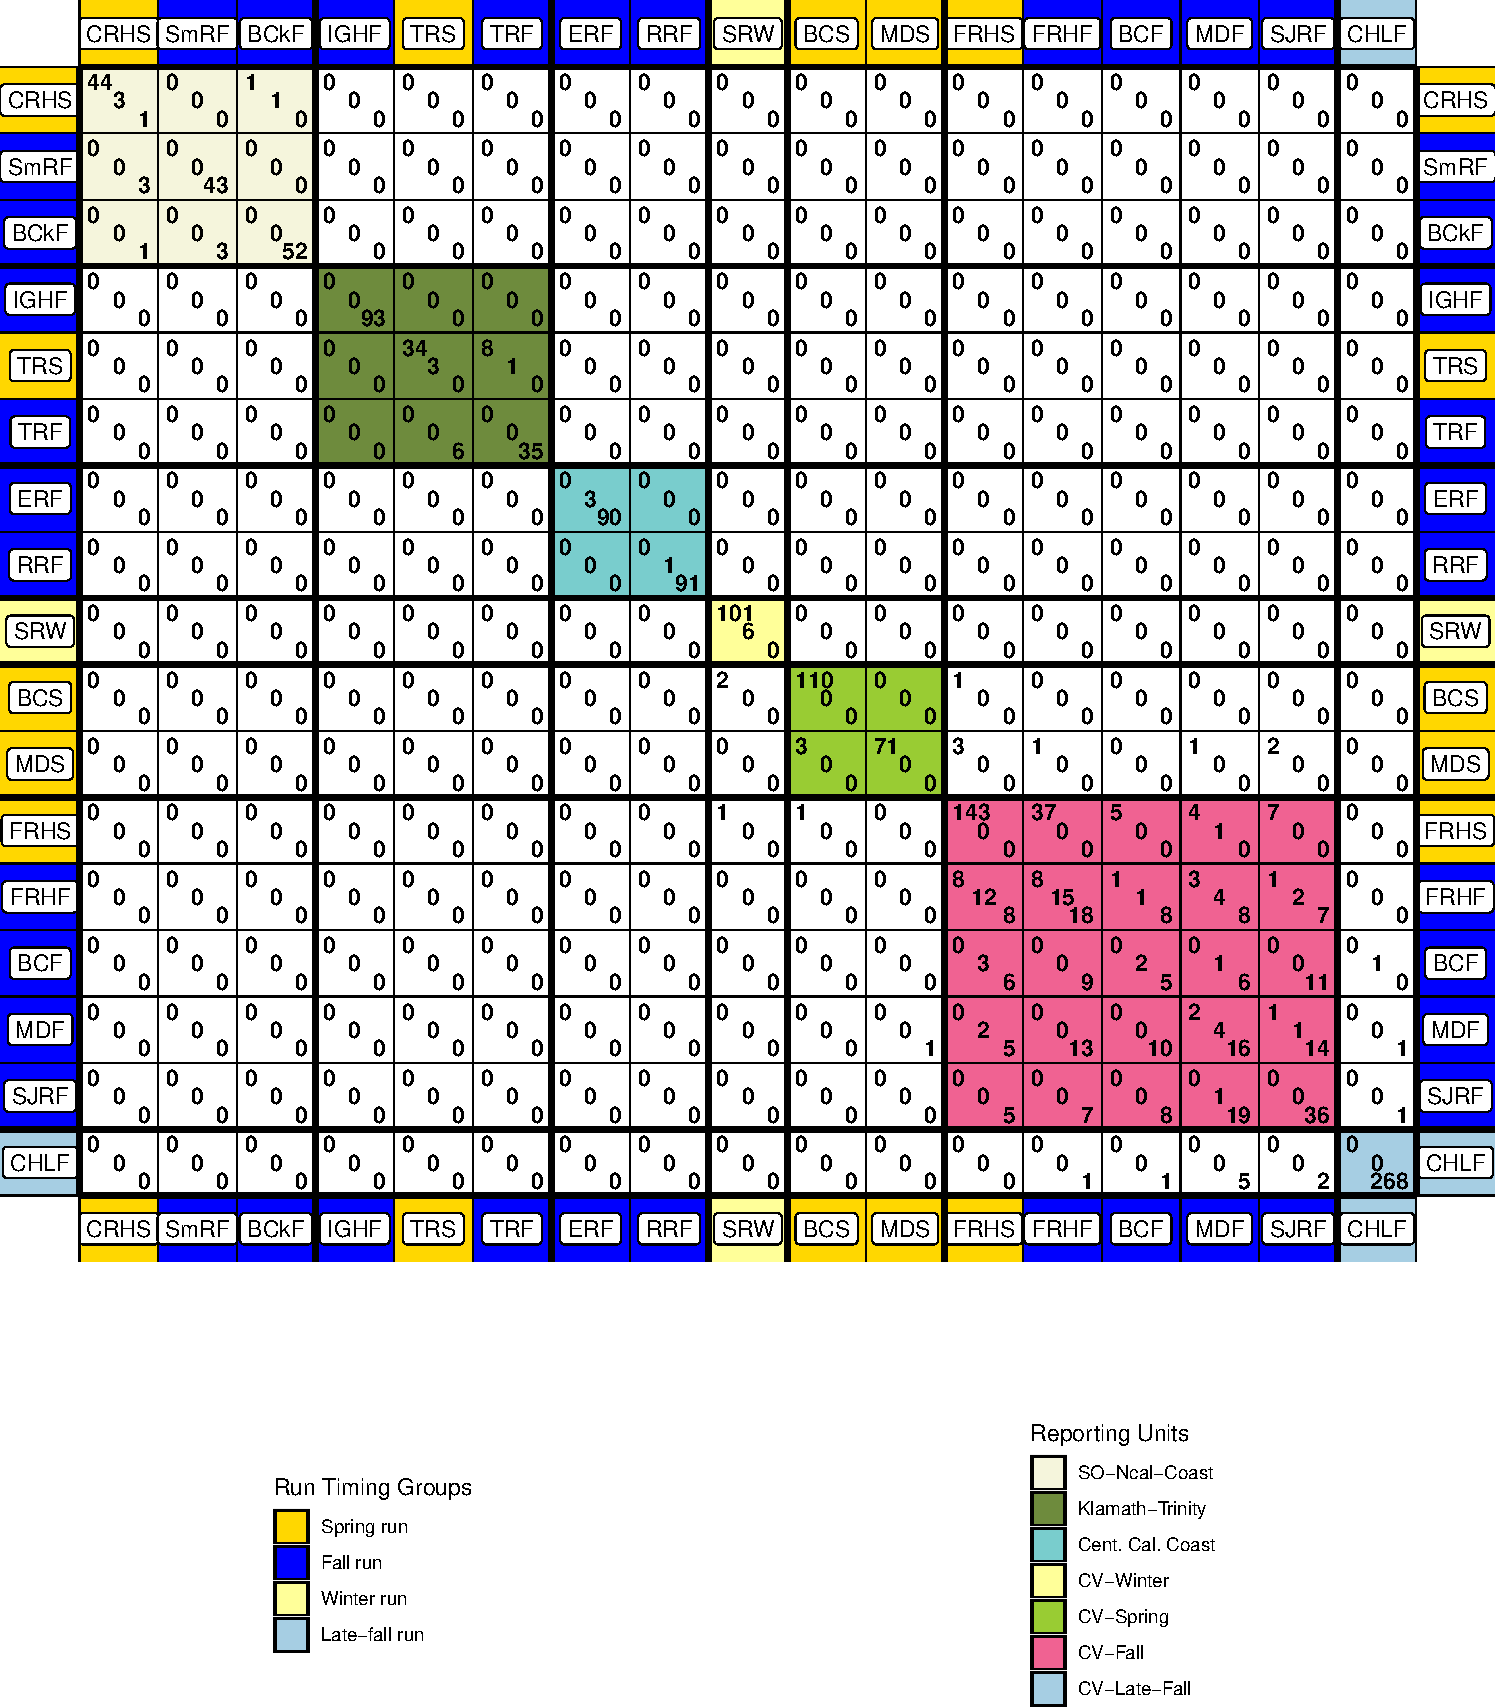
\includegraphics[width=0.8\textwidth]{images/rosa-gsi-table-crop.pdf}
\end{center}
\caption[Assignment table by RoSA genotype]{\footnotesize Assignment table
like that in Figure~\ref{fig:gsi}b in the paper, but with numbers according to genotypes
at the RoSA. In each cell, the top left entry gives the number of EE (early run allele homozygotes)
genotypes, the middle entry is the number of EL genotypes (heterozygotes), and the bottom
right entry gives the number of LL (late-run homozygote) genotypes. }
\label{fig:rosa-gsi}
\end{figure}
%%%%%%%%%%%%%%%%%%%%



%%%%%%%%%%%%%%%%%%%%%% 
\begin{figure}
\begin{center}
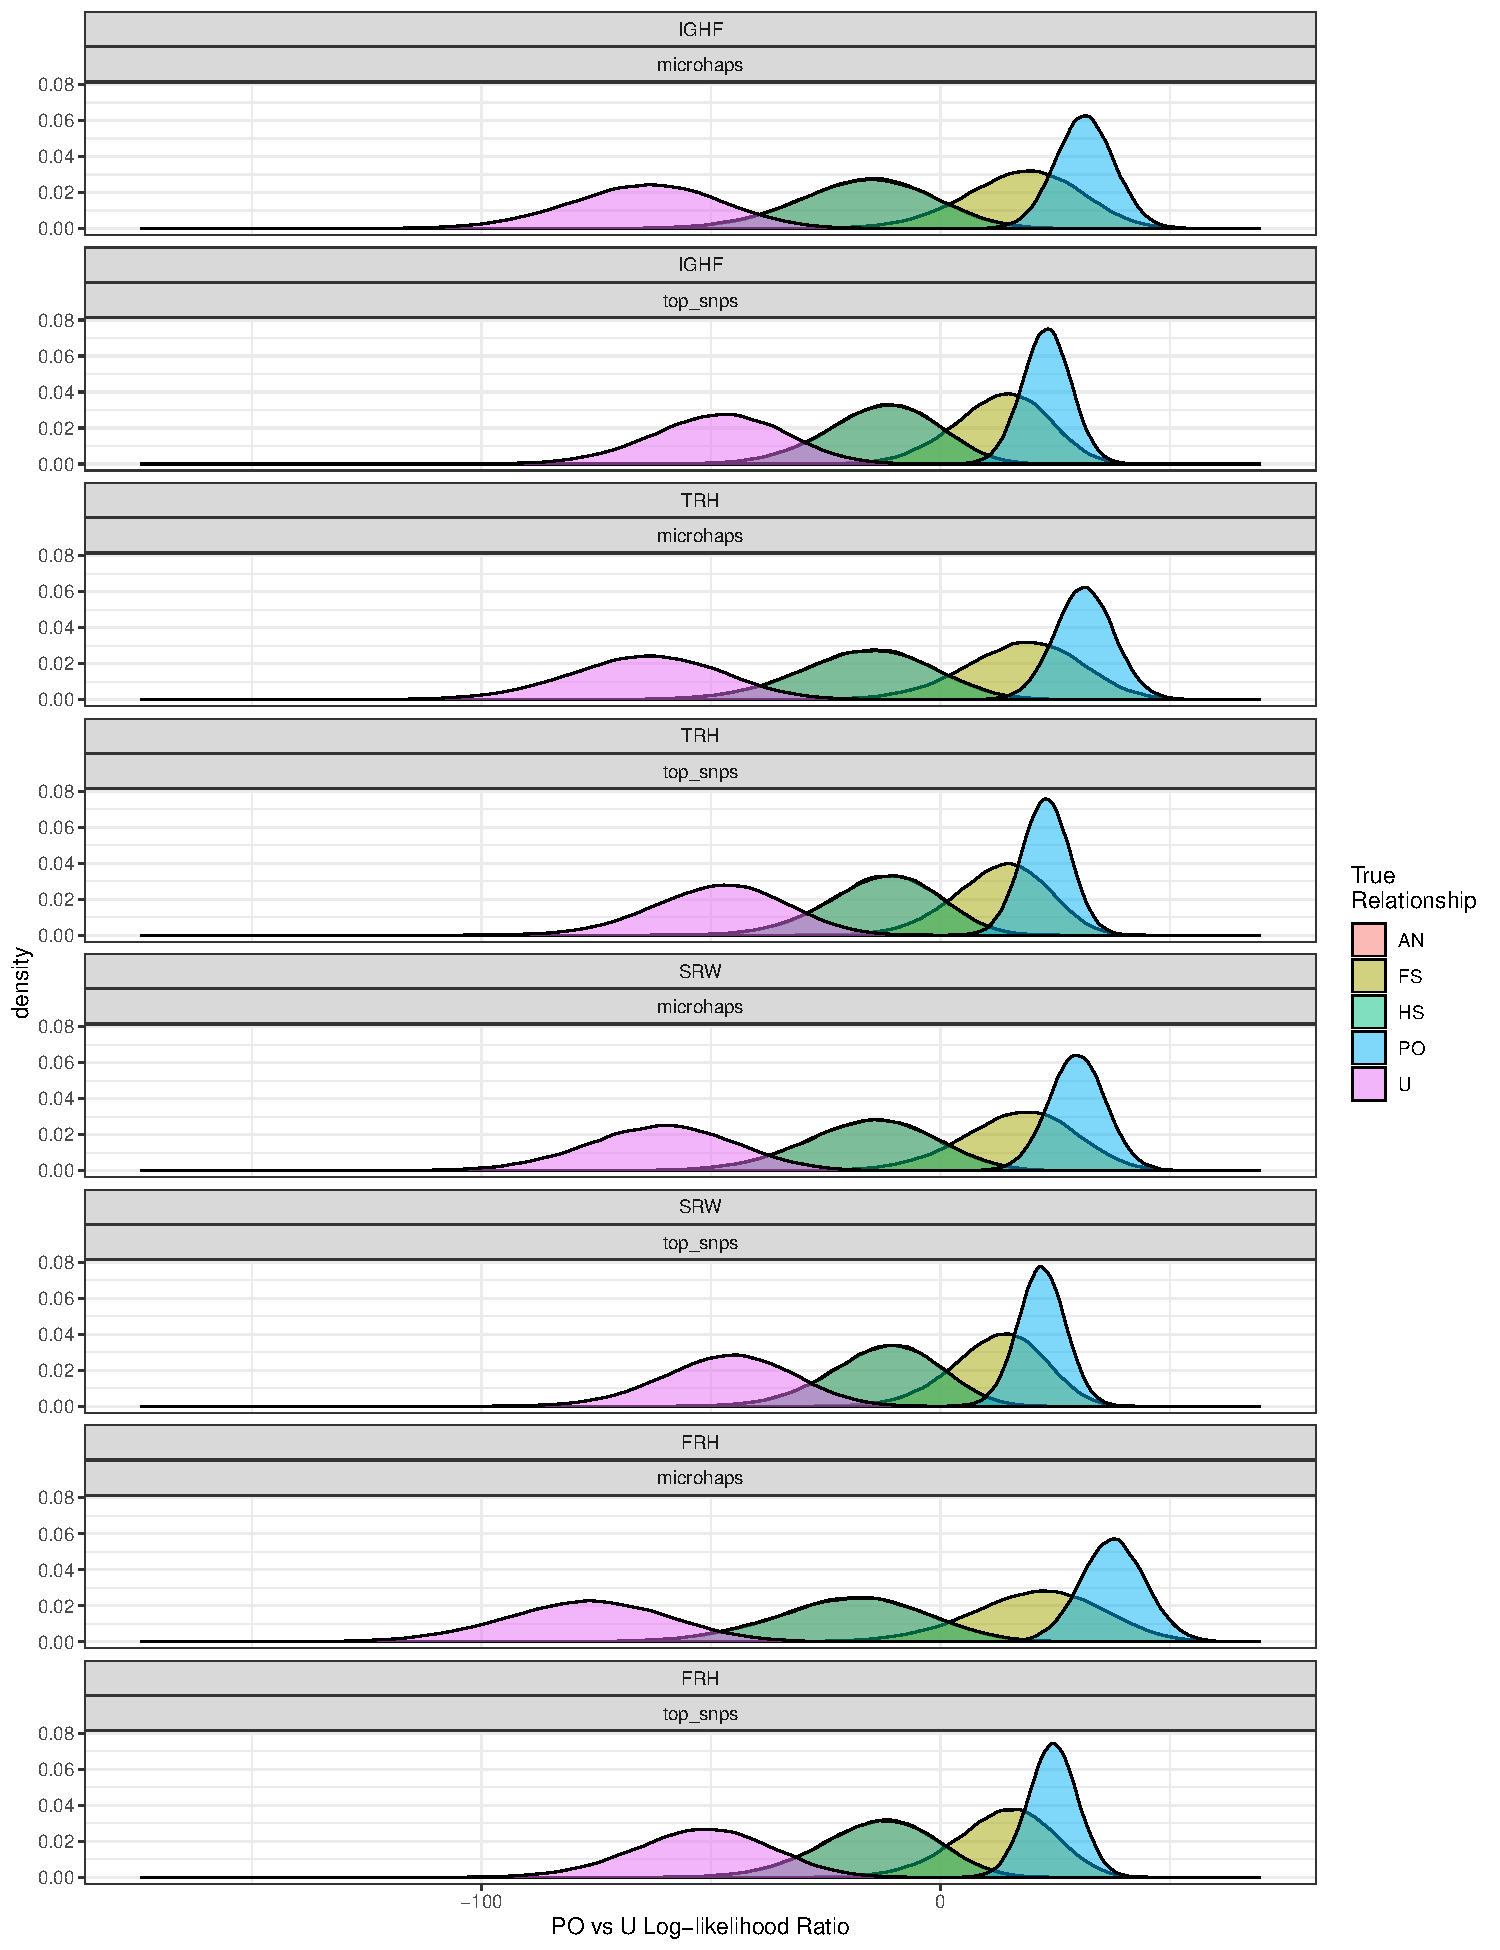
\includegraphics[width=0.9\textwidth]{images/ckmr-comp-figure-crop.pdf}
\end{center}
\caption[Comparison of microhaplotypes vs.~best SNP in each amplicon]{\footnotesize 
A comparison of the distribution of log-likelihood ratios when using all the alleles at each
amplicon typed as microhaplotypes ("microhaps" in the panel headers) versus using just a single (the most informative) SNP from each
amplicon ("top\_snps" in the panel headers).  Results shown for four hatchery collections in California 
(FRH: Feather River Hatchery [spring and fall]; IGH: Iron Gate Hatchery; SRW: Sacramento Winter Run;
TRH: Trinity River Hatchery [spring and fall]).  The density plots show
the distribution of log-likelihood ratios for Parent-Offspring vs Unrelated for four different relationships:
PO = parent offspring; FS = full-sibling; HS = Half sibling; AN = avuncular (i.e., aunt-niece, etc.)
The distributions for AN and HS overlap completely.  Note that the overlap between FS and PO occurs
for the PO vs U likelihood ratio, but is nearly eliminated with the PO vs FS likelihood ratio, allowing these
two relationships to be resolved accurately.}
\label{fig:ckmr-comp}
\end{figure}
%%%%%%%%%%%%%%%%%%%%




%%%%%%%%%%%%%%%%%%%
\begin{figure}
\includegraphics[width=\textwidth]{images/winter-v-non-winter-mh-plot_nind_ge10.pdf}
\caption[
	Absolute difference in allele frequency between winter run and non-winter run fish
]{
	\footnotesize Absolute difference in allele frequency between winter run and non-winter run fish of the CCV.
	The plot shows only those SNPs with at least a frequency difference of 0.5 between the two groups. Each point
	is a SNP. The  $x$ axis shows position in the Otsh\_v1.0 genome
	with color alternating by chromosome as indicated by RefSeq names on plot.
}
\label{fig:wrap-absdiff}
\end{figure}



%%%%%%%%%%%%%%%%%%%
\begin{figure}
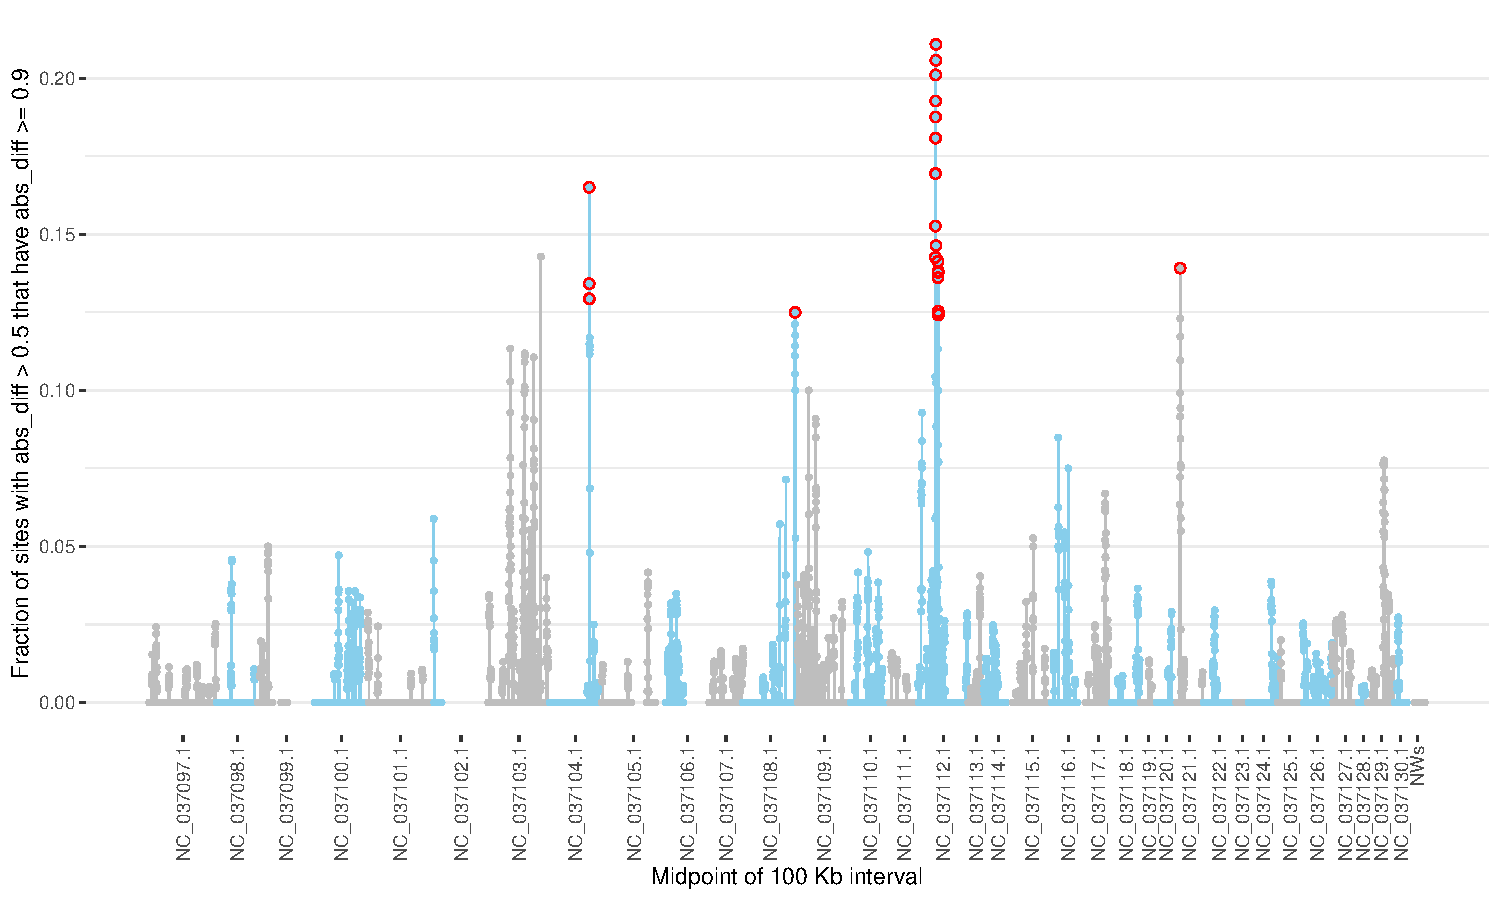
\includegraphics[width=\textwidth]{images/wrap-slide-window.pdf}
\caption[
	Sliding windows of absolute allele frequency difference between winter run and others
]{
	\footnotesize Values within 100 kb sliding windows of the fraction of sites with $|d|$ (absolute difference in
	allele frequency between winter run and non-winter run fish of the CCV) greater than 0.5 that also have
	$|d|>0.9$. The  $x$ axis shows position in the Otsh\_v1.0 genome
	with color alternating by chromosome as indicated by RefSeq names on plot. Red circles denote sliding
	windows chosen for further investigation for candidate markers.
}
\label{fig:wrap-slide-window}
\end{figure}





%%%%%%%%%%%%%%%%%%%
\begin{figure}
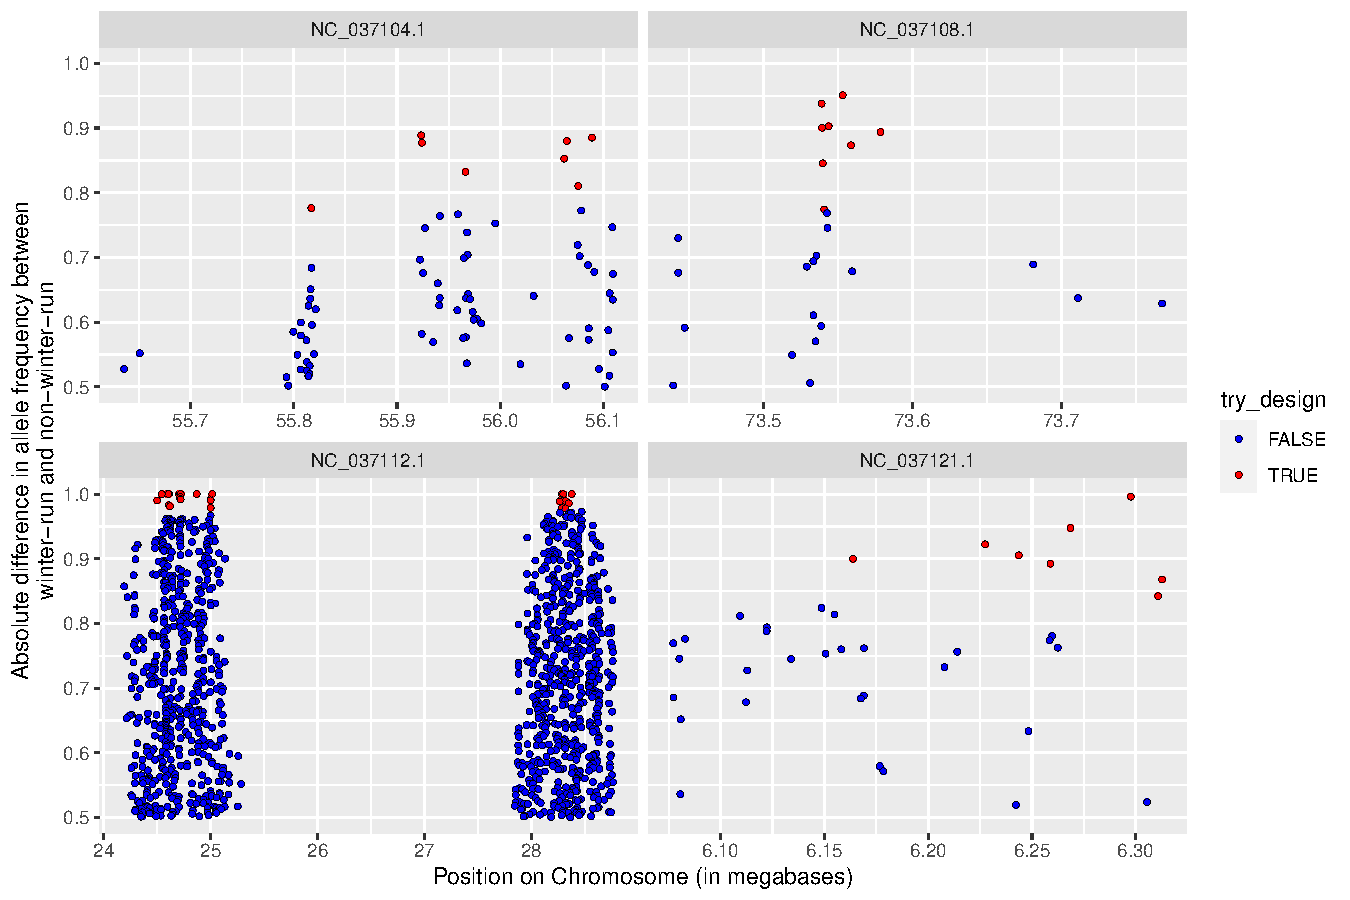
\includegraphics[width=\textwidth]{images/wrap-candi.pdf}
\caption[
	61 candidates for primer design for winter-run-associated polymorphisms
]{
	\footnotesize Genomic positions and values of $|d|$ (absolute difference in
	allele frequency between winter run and non-winter run fish of the CCV)
	for the 61 candidate SNPs (in red) to design for winter-run-associated polymorphisms
	(WRAPs).  Other sites are shown in blue.  The $x$-axis shows position on
	each chromsome in the Otsh\_v1.0 assembly.  The chromsome name is indicated in the facet headers by
	RefSeq name
}
\label{fig:wrap-candi}
\end{figure}

